\chapter{Results}

\begin{figure}
    \centering
    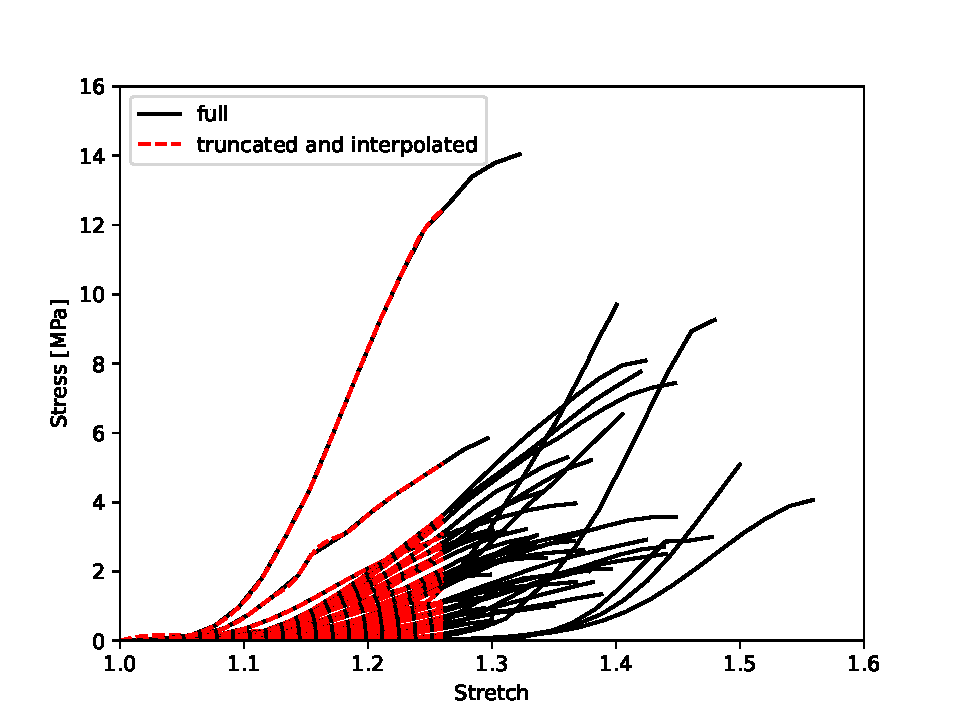
\includegraphics[width=\linewidth]{skinstression/images/truncated-and-interpolated-curves.pdf}
    \caption[Truncated and spline interpolated curves]{
        The strain-stress curves (black) were truncated and interpolated (dotted red)
        using non-uniform, interpolating splines on the stretch values of the curve with the lowest maximum stretch.
    }
    \label{fig:trunc_interp_curves}
\end{figure}

\section{Participants}

Earlier studies (refs) include 18 individuals (5 men, 4 women, and 6 unknown).
Abdomen data was excluded, because the strain-stress curves differ significantly from the thigh.
All thigh data is included, which is different from the original study, where only the 48 latest samples were used.
These considerations result in data including 15 individuals (5 men, 4 women, 3 unknown).
Ages range from 61 to 94.
Skin tissue is cut from the thigh and cut in multiple pieces of roughly the same shape.\marginpar{protocol?}
From every skin tissue piece, strain-stress curves are measured.
The number of measured strain-stress curves range from 1 to 13.
The source of data is summarized in table~\ref{tab:source_of_data}
\begin{table}
    \centering
    \caption[Source of data]{
        The selected individuals and their sex, age and number of strain-stress curves.
        - denotes unknown data.
    }
    \label{tab:source_of_data}
    \begin{tabular}{lllr}
        \toprule
        person & sex    & age & \# curves \\
        \midrule
        4      & -      & -   & 1         \\
        5      & male   & 61  & 1         \\
        6      & male   & 66  & 2         \\
        7      & male   & 79  & 1         \\
        8      & male   & 77  & 1         \\
        9      & male   & 75  & 1         \\
        10     & female & 94  & 1         \\
        11     & -      & -   & 1         \\
        12     & -      & -   & 1         \\
        13     & male   & 82  & 3         \\
        14     & female & 90  & 4         \\
        15     & female & 87  & 5         \\
        16     & male   & 95  & 12        \\
        17     & male   & 83  & 13        \\
        18     & female & 88  & 9         \\
        \bottomrule
    \end{tabular}
\end{table}

\section{Predictor pre-selection}
\subsection{Exponential}
An exponential fit to \cref{eq:exp} is shown in \cref{fig:exp_fits}.
$R^2 = \num{0.9497}$.
The exponent is not able to fit the plateau that is often exhibited near maximum stretch.

\begin{figure}
    \centering
    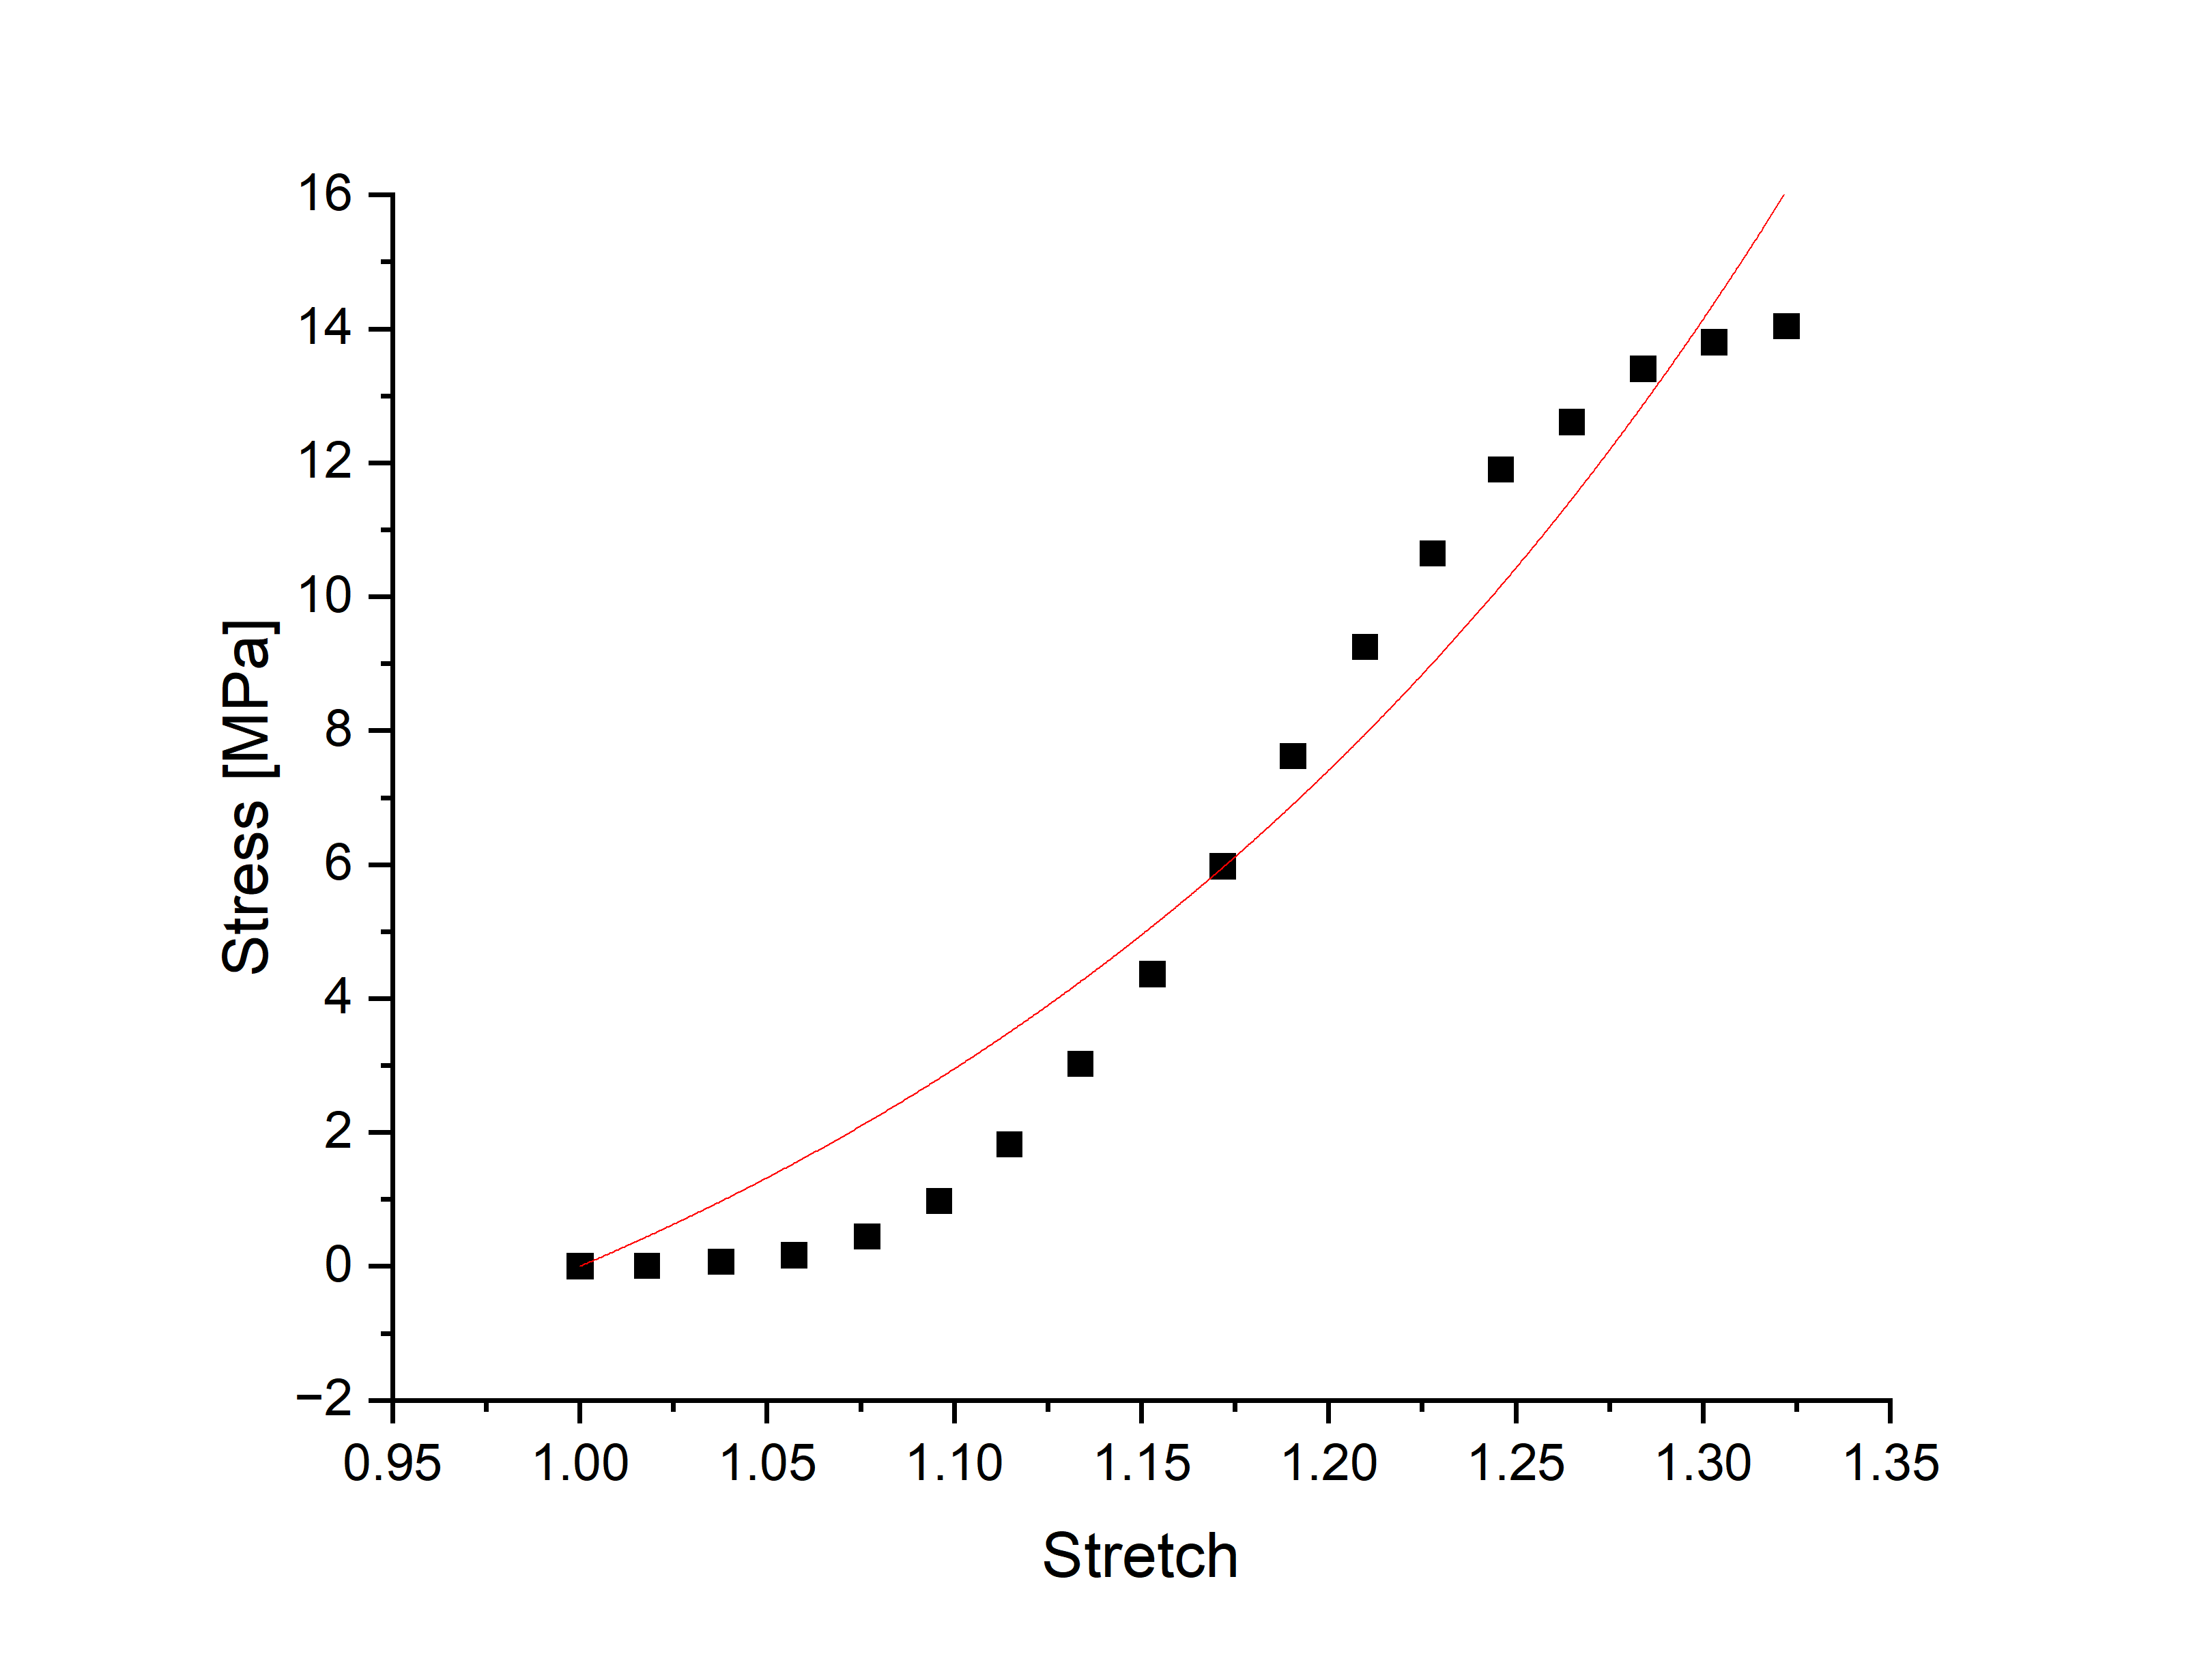
\includegraphics[width=0.5\linewidth]{skinstression/images/exp-fits/exponential.png}
    \caption[Exponential fit]{
        Exponential fit with \cref{eq:exp} (red) for one stress-strain curve (black).
        Fit parameters were $G_0=\qty{23.8\pm4.0}{\mega\pascal\per\stretch}$, and $\lambda=\qty{4.1\pm 1.0}{\stretch}$.
        $R^2=\num{0.9497}$.
    }
    \label{fig:exp_fits}
\end{figure}

\subsection{PCA}
The PCA fit for every truncated and interpolated strain-stress curve is depicted in \cref{fig:pca_fits}.
For every fit, $R^2$ is calculated with respect to the interpolated and truncated data.
On average, $\overline{R^2} \approx \num{0.9927 \pm 0.0022}$.
Due to the nature of PCA, the exponential part of the slower curves is not included in the making of the fit.

\begin{figure*}
    \centering
    \foreach \c in {1,2,...,61}{%
            \IfFileExists{skinstression/images/pca-fits/sample_\c.pdf} {%
                \includegraphics[width=0.24\linewidth]{skinstression/images/pca-fits/sample_\c.pdf}
            }{%
                % files do not exist, so nothing to do
            }
        }
    \caption[PCA fits]{
        PCA fits for every truncated and interpolated strain-stress curve.
        The interpolated measurements (blue) are estimated by the PCA curve (red) along with their $R^2$.
        PCA is done on all available thigh data.
        Note that the vertical axes are not equal.
    }
    \label{fig:pca_fits}
\end{figure*}

\subsection{Logistic curve}
The logistic curve fit for every strain-stress curve is shown in \cref{fig:logistic_fits}.
For every fit, $R^2$ is calculated.
On average, $\overline{R^2} \approx \num{0.9979 \pm 0.0039}$.

\begin{figure*}
    \centering
    \foreach \c in {1,2,...,61}{%
            \IfFileExists{skinstression/images/logistic-fits/sample_\c.pdf} {%
                \includegraphics[width=0.24\linewidth]{skinstression/images/logistic-fits/sample_\c.pdf}
            }{%
                % files do not exist, so nothing to do
            }
        }
    \caption[Logistic fits]{
        Logistic fits (red) and their $R^2$ for every strain-stress curve (black).
        Note that the vertical axes are not equal.
    }
    \label{fig:logistic_fits}
\end{figure*}

Because the logistic curve describes the stress-strain data more accurate than PCA or the exponential, it will be used from now on.

%%%%%%%%%%%%%%%%%%%%%%%%%%%%%%%%%%%%
% HYPERPARAMETER SEARCH
%%%%%%%%%%%%%%%%%%%%%%%%%%%%%%%%%%%%

\section{Hyperparameter optimization}

\subsection{Search 1, without Yeo-Johnson transform}
The contour plot is shown in \cref{fig:skinstression-search1-contour}.
Only the loss curves of the best trial (71) is shown in \cref{fig:skinstression-search1-best-loss}.
Both training and validation loss show an increase at the learning rate restarts.

\begin{figure}
    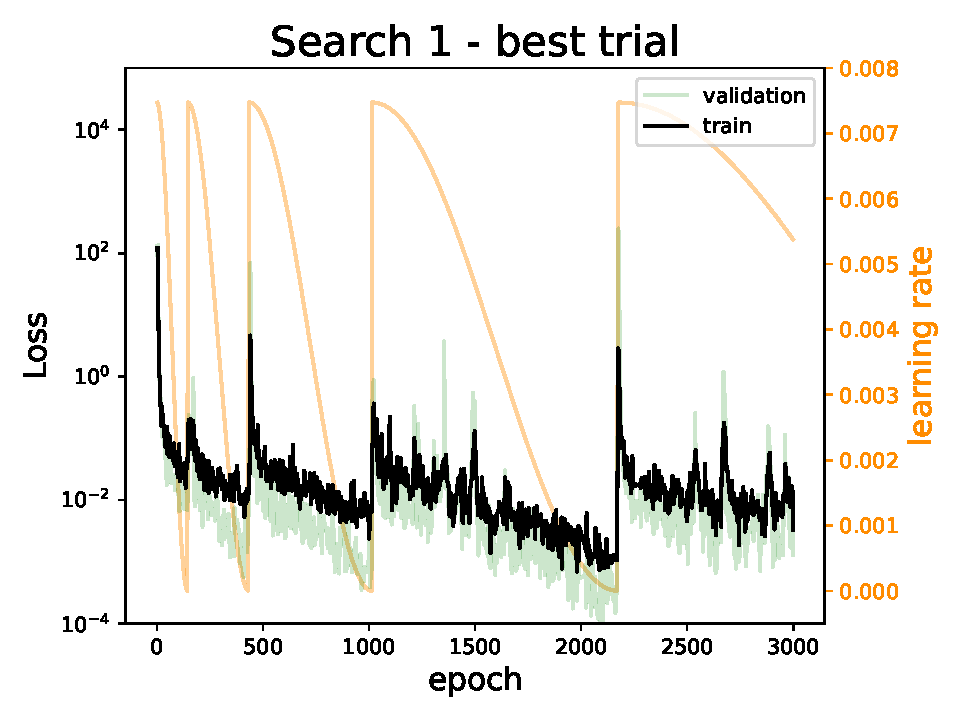
\includegraphics[]{skinstression/images/hyperparameter-search/search-1/best-trial-loss.pdf}
    \caption[Best loss curve of search 1]{
        Successive halving trial 71 of 100 has shown the best loss for search 1.
        The training loss (black) is followed by the validation loss (light green).
        The learning rate (orange) restarts explain sudden increase in loss.
    }
    \label{fig:skinstression-search1-best-loss}
\end{figure}

\begin{figure*}
    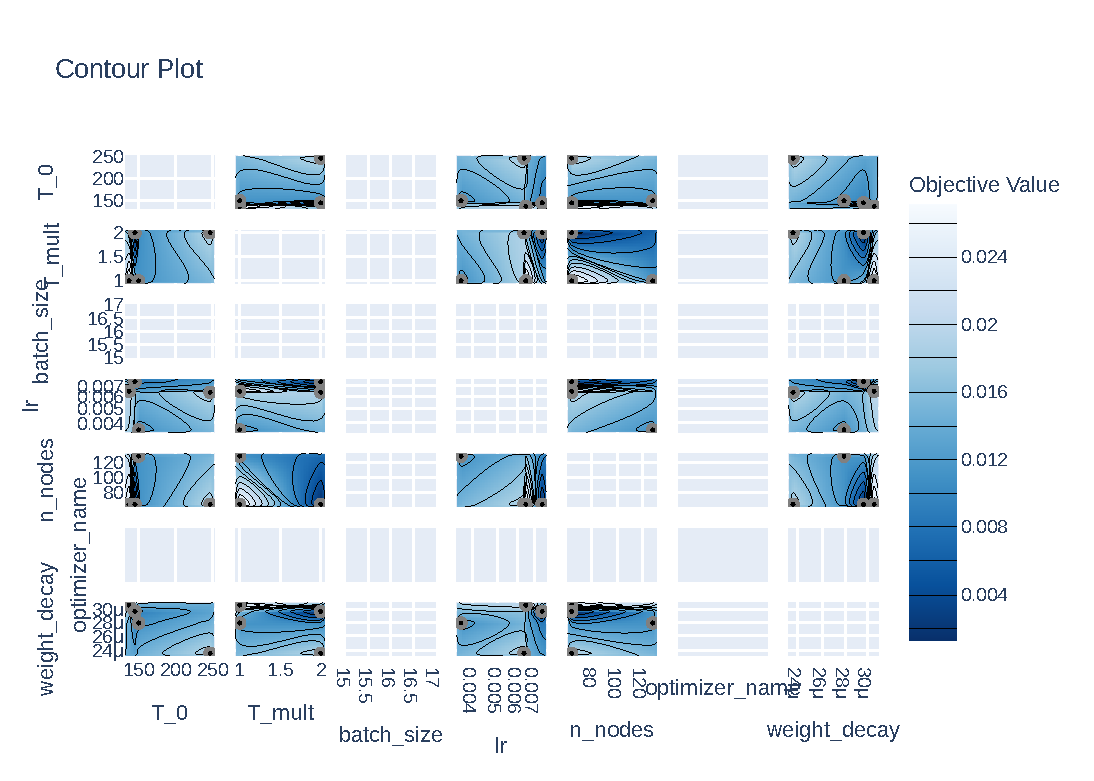
\includegraphics[angle=90,width=0.9\textheight, height=\linewidth,keepaspectratio]{skinstression/images/hyperparameter-search/search-1/contour.pdf}
    \caption[Search 1 contour plot]{
        Contour plot of search 1.
        Darker regions denote better results.
        This contour plot is only constructed from trials which have not been pruned.
    }
    \label{fig:skinstression-search1-contour}
\end{figure*}

\subsection{Search 2, without Yeo-Johnson transform}
The contour plot is shown in \cref{fig:skinstression-search2-contour}.
Only the loss curves of the best trial (184) is shown in \cref{fig:skinstression-search2-best-loss}.
Both training and validation loss show an increase at the learning rate restarts.

\begin{figure}
    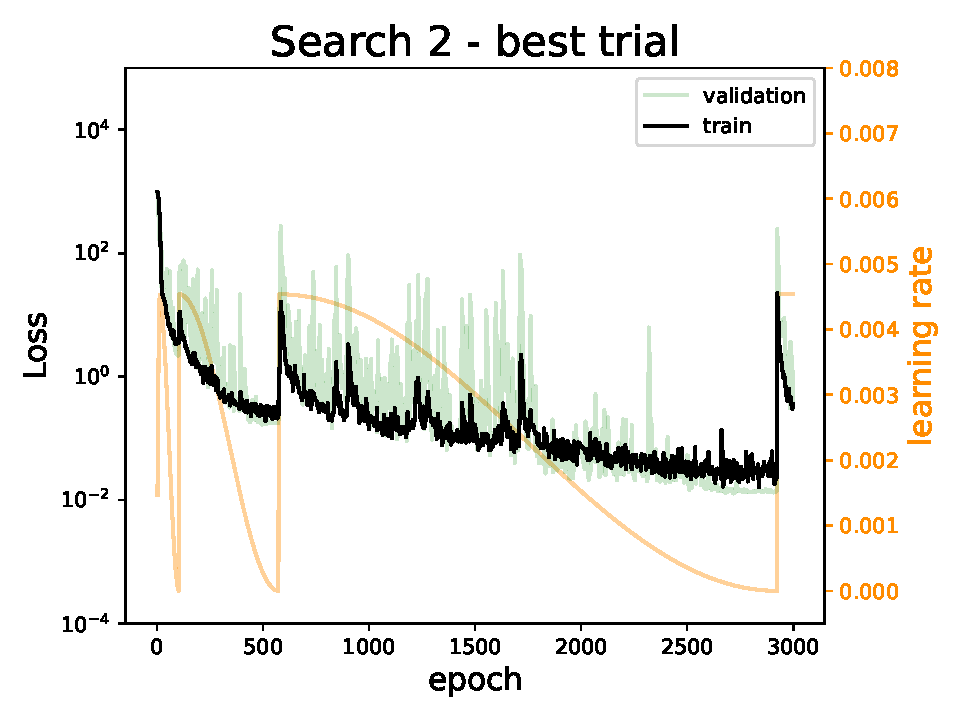
\includegraphics[]{skinstression/images/hyperparameter-search/search-2/best-trial-loss.pdf}
    \caption[Best loss curve of search 2]{
        Hyperband trial 184 of 300 has shown the best loss for search 2.
        The training loss (black) is followed by the validation loss (light green).
        The learning rate (orange) restarts explain sudden increase in loss.
    }
    \label{fig:skinstression-search2-best-loss}
\end{figure}

\begin{figure*}
    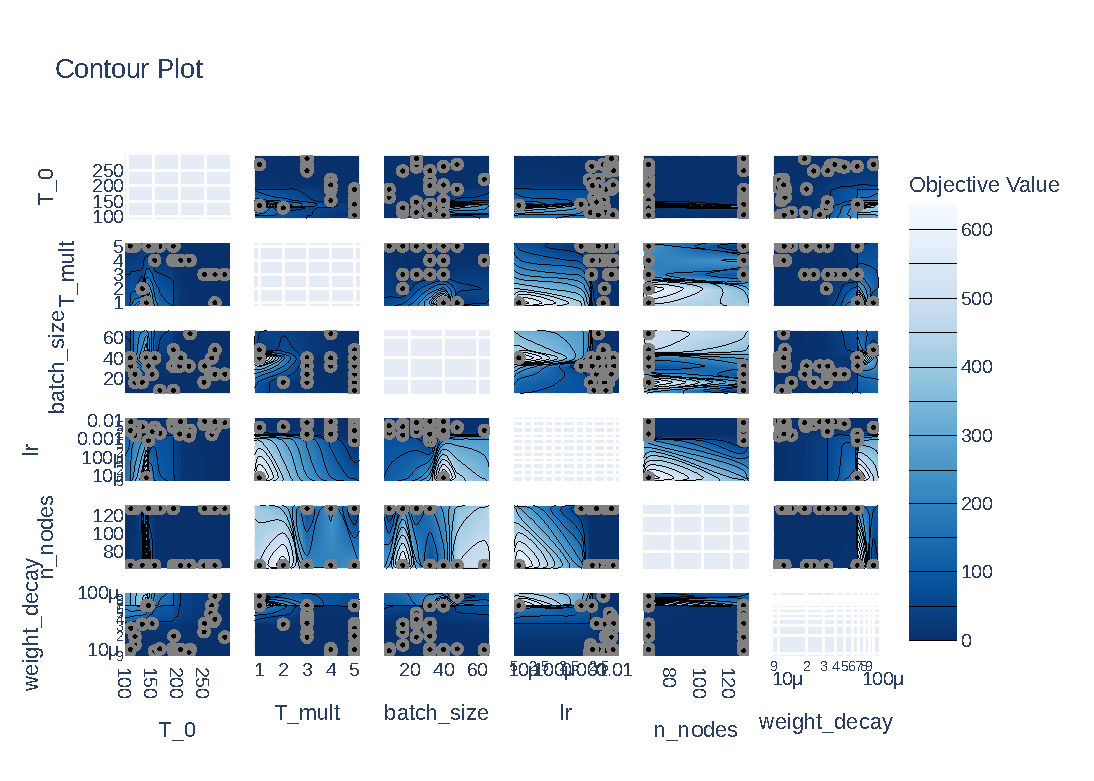
\includegraphics[angle=90,width=0.9\textheight, height=\linewidth,keepaspectratio]{skinstression/images/hyperparameter-search/search-2/contour.pdf}
    \caption[Search 2 contour plot]{
        Contour plot of search 2.
        Darker regions denote better results.
        This contour plot is only constructed from trials which have not been pruned.
    }
    \label{fig:skinstression-search2-contour}
\end{figure*}

\subsection{Search 3, with Yeo-Johnson transform}
The contour plot is shown in \cref{fig:skinstression-search3-contour}.
Only the loss curves of the best trial (73) is shown in \cref{fig:skinstression-search3-best-loss}.
The training and validation losses diverge, showing the model overfits.

\begin{figure}
    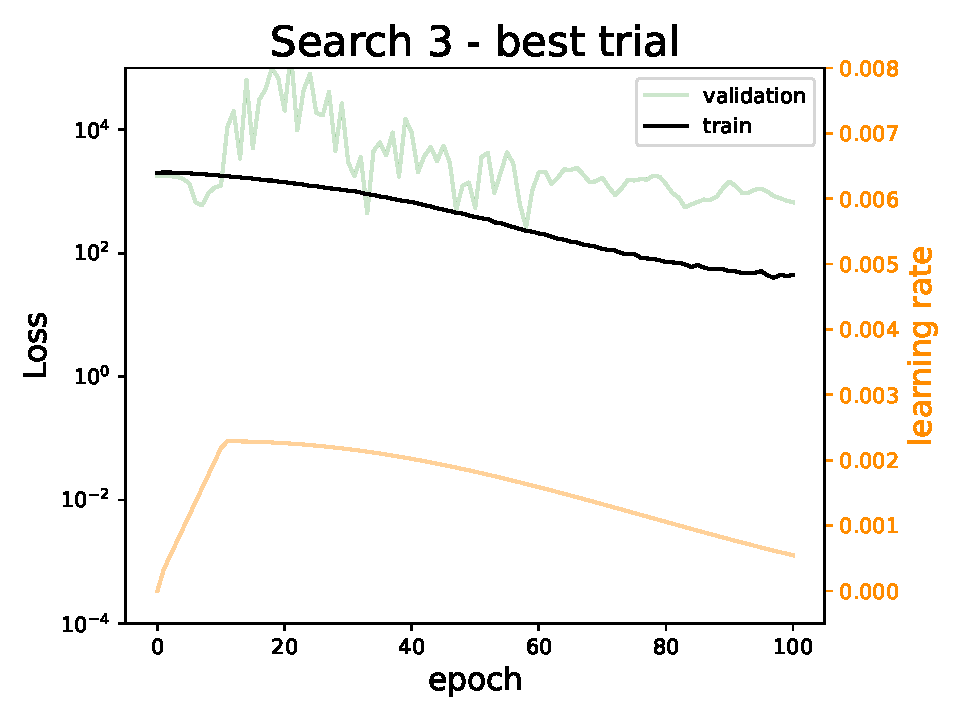
\includegraphics[]{skinstression/images/hyperparameter-search/search-3/best-trial-loss.pdf}
    \caption[Best loss curve of search 3]{
        Hyperband trial 73 of 300 has shown the best loss for search 3.
        The training loss (black) and the validation loss (light green) diverge.
        The learning rate (orange).
        The trial was pruned at epoch 100.
    }
    \label{fig:skinstression-search3-best-loss}
\end{figure}

\begin{figure*}
    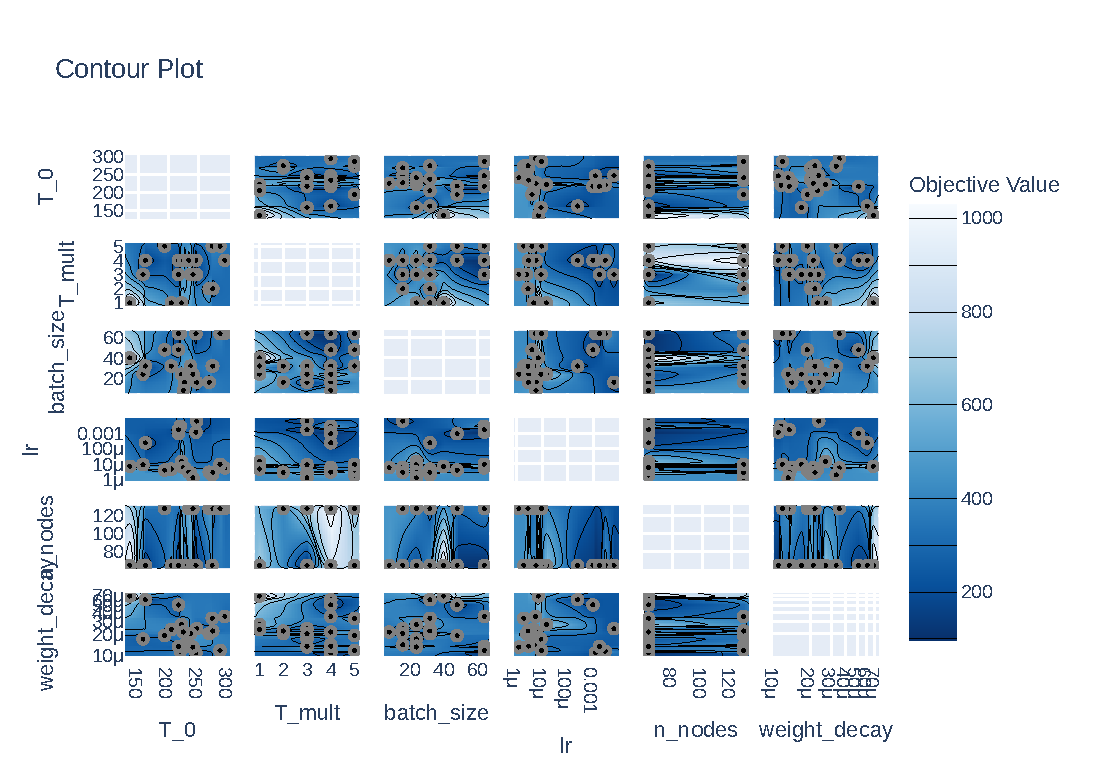
\includegraphics[angle=90,width=0.9\textheight, height=\linewidth,keepaspectratio]{skinstression/images/hyperparameter-search/search-3/contour.pdf}
    \caption[Search 3 contour plot]{
        Contour plot of search 3.
        Darker regions denote better results.
        This contour plot is only constructed from trials which have not been pruned.
    }
    \label{fig:skinstression-search3-contour}
\end{figure*}

%%%%%%%%%%%%%%%%%%
% TRAINING
%%%%%%%%%%%%%%%%%%
\section{Training}
Search 1 without the Yeo-Johnson transform yields a lower loss.
The corresponding hyperparameters are used for further training.

